\section{Finite State Machine Authoring Tools}
\label{sec: app-dev-statemachine}

\begin{figure}[t]
    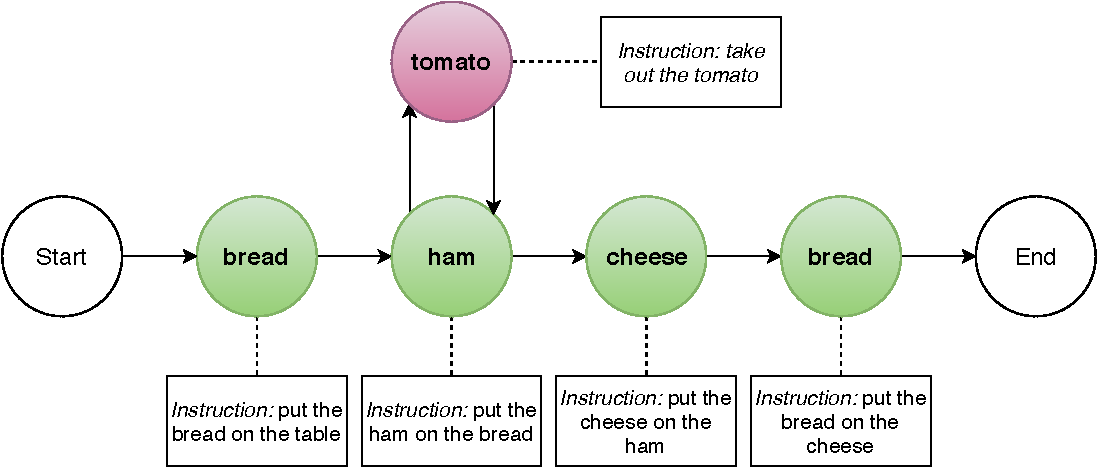
\includegraphics[width=\linewidth]{FIGS/state_transition_4.pdf}
    \caption{An example finite state machine (FSM) for the application that assists in making a sandwich. White circles represent start and end states of the process. Green circles represent correct states that help the user finish the task. The red circle represents an error state that requires the user to recover to the latest correct state to finish the task.}
    \label{fig:sme}
\end{figure}

To develop a Gabriel application for a particular task, developers typically
have to write custom code. This process gives them flexibility, but it takes a
significant amount of time. We chose to offer higher-level abstractions that
allow people to create applications quickly while still having some flexibility.

We observed that the implementation of a cognitive assistant mainly consists of
components to identify user states using computer vision models, specify
instructions to users based on the current state, and keep track of progress on
the task. We created a a workflow modeling tool, SME, which can transform the
process of completing a task into a specific model, substantially reducing the
expert modeling effort required. By using a framework to reason about
step-by-step application, along with workflow information from WE and object
recognition models from TPOD, SME also automatically generates a Gabriel
executable application based on the modeled workflow.

%Finite state machines (FSMs) have commonly been used to model business processes~\cite{borger2007modeling} and activities. A computer application can be synthesized based on a FSM~\cite{ali1998object, niaz2005automatic, bjoraa2000generating}.
The applications SME generates are defined by a set of steps. Each state
corresponds to the subset of steps that a user has completed. We use a FSM to
keep track of the current state of a task and the future states that we should
transition to when a user takes a certain action. Transitions among states are
triggered by visual changes resulting from user actions. For example, the user
might put a piece of ham on top of a piece of bread. In addition, each state has
its own processing functions, which convert the current visual state into
information that the application can understand. We provide a list of
pre-defined processing functions, such as object detection DNNs. Task experts
also have the flexibility to add custom processing functions when needed.
Figure~\ref{fig:sme} shows a sample workflow as a finite state machine. Once the
task expert finalizes a FSM, SME automatically compile the FSM to generate an
executable application.
%We also plan to integrate state machines in Ajalon to model working processes.